\begin{blocksection}
\question What does it mean for a filter to be shift-invariant?

\begin{solution}[0.75in]
If a filter is shift-invariant, it will perform the same high-level computation (e.g. taking a median of a neighborhood) no matter which part of the signal it is being applied to. The filter will do the same thing no matter where we put it.

Mathematically, this means $[I(x, y) * f](x - n, y - k) = [I(x - n, y - k) * f](x, y)$.
\end{solution}
\end{blocksection}

%%%

\begin{blocksection}
\question Convolve the image $\mb{F}$ with filter $\mb{h}$. Assume ones beyond the boundaries. 

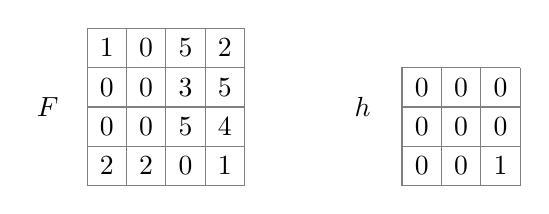
\begin{tikzpicture}
\node at (-1.5, 0) {$\mb{F}$};
\draw[step=0.5cm, color=gray] (-1, -1) grid (1, 1);
\node at (-0.75, +0.75) {1};
\node at (-0.25, +0.75) {0};
\node at (+0.25, +0.75) {5};
\node at (+0.75, +0.75) {2};
\node at (-0.75, +0.25) {0};
\node at (-0.25, +0.25) {0};
\node at (+0.25, +0.25) {3};
\node at (+0.75, +0.25) {5};
\node at (-0.75, -0.25) {0};
\node at (-0.25, -0.25) {0};
\node at (+0.25, -0.25) {5};
\node at (+0.75, -0.25) {4};
\node at (-0.75, -0.75) {2};
\node at (-0.25, -0.75) {2};
\node at (+0.25, -0.75) {0};
\node at (+0.75, -0.75) {1};

\node at (2.5, 0) {$\mb{h}$};
\draw[step=0.5cm, color=gray] (2.99, -1) grid (4.5, 0.5);
\node at (3.25, +0.25) {0};
\node at (3.75, +0.25) {0};
\node at (4.25, +0.25) {0};
\node at (3.25, -0.25) {0};
\node at (3.75, -0.25) {0};
\node at (4.25, -0.25) {0};
\node at (3.25, -0.75) {0};
\node at (3.75, -0.75) {0};
\node at (4.25, -0.75) {1};
\end{tikzpicture}

\begin{solution}[0.75in]
\begin{center}
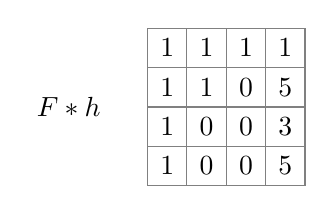
\begin{tikzpicture}
\node at (-2, 0) {$\mb{F} * \mb{h}$};
\draw[step=0.5cm, color=gray] (-1, -1) grid (1, 1);
\node at (-0.75, +0.75) {1};
\node at (-0.25, +0.75) {1};
\node at (+0.25, +0.75) {1};
\node at (+0.75, +0.75) {1};
\node at (-0.75, +0.25) {1};
\node at (-0.25, +0.25) {1};
\node at (+0.25, +0.25) {0};
\node at (+0.75, +0.25) {5};
\node at (-0.75, -0.25) {1};
\node at (-0.25, -0.25) {0};
\node at (+0.25, -0.25) {0};
\node at (+0.75, -0.25) {3};
\node at (-0.75, -0.75) {1};
\node at (-0.25, -0.75) {0};
\node at (+0.25, -0.75) {0};
\node at (+0.75, -0.75) {5};
\end{tikzpicture}
\end{center}
\end{solution}
\end{blocksection}

%%%

\begin{blocksection}
\question Match the images to the descriptions.

\begin{figure}[H]
\includegraphics[width=0.75\textwidth]{airplane}
\end{figure}

\begin{solution}[0.75in]
From top to bottom: \textit{filtered with $\begin{bmatrix}\begin{bmatrix}1, -1\end{bmatrix}\end{bmatrix}$ kernel}, \textit{filtered with Gaussian kernel}, \textit{filtered with $\begin{bmatrix}\begin{bmatrix}1\end{bmatrix}, \begin{bmatrix}-1\end{bmatrix}\end{bmatrix}$ kernel}, \textit{original image}.
\end{solution}
\end{blocksection}

%%%

\begin{blocksection}
\question One application of filtering/convolution is template matching: finding regions in an image that are similar to a given patch. How would you imagine that this is done?

\begin{solution}[0.75in]
Convolve the image with the (flipped) patch. In the resulting image, a high brightness at a pixel means that the patch is very similar to the neighborhood around that pixel.
\end{solution}
\end{blocksection}

%%%

\begin{blocksection}
\question Give a $3 \times 3$ linear filter that shifts an image one pixel to the right and increases the image brightness by 50\%.

\begin{solution}[0.75in]
\begin{center}
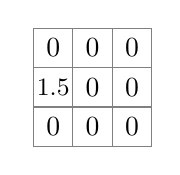
\begin{tikzpicture}
\draw[step=0.5cm, color=gray] (2.99, -1) grid (4.5, 0.5);
\node at (3.25, +0.25) {0};
\node at (3.75, +0.25) {0};
\node at (4.25, +0.25) {0};
\node at (3.25, -0.25) {{\small 1.5}};
\node at (3.75, -0.25) {0};
\node at (4.25, -0.25) {0};
\node at (3.25, -0.75) {0};
\node at (3.75, -0.75) {0};
\node at (4.25, -0.75) {0};
\end{tikzpicture}\: assuming correlation,\:\:\:
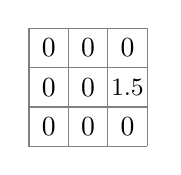
\begin{tikzpicture}
\draw[step=0.5cm, color=gray] (2.99, -1) grid (4.5, 0.5);
\node at (3.25, +0.25) {0};
\node at (3.75, +0.25) {0};
\node at (4.25, +0.25) {0};
\node at (3.25, -0.25) {0};
\node at (3.75, -0.25) {0};
\node at (4.25, -0.25) {{\small 1.5}};
\node at (3.25, -0.75) {0};
\node at (3.75, -0.75) {0};
\node at (4.25, -0.75) {0};
\end{tikzpicture}\: assuming convolution.
\end{center}
\end{solution}
\end{blocksection}

%%%

\begin{blocksection}
\question How do you obtain an edge image if you're only allowed a blurring filter?

\begin{solution}[0.75in]
Apply the blurring filter, then subtract the result from the original image. (The blurred image represents low frequencies. After subtracting these out, we are left with the high frequencies.)
\end{solution}
\end{blocksection}
